\documentclass[11pt,ngerman]{article}
\usepackage{geometry}
\usepackage[T1]{fontenc}
\usepackage[utf8]{inputenc}
\usepackage{babel}
\usepackage{lmodern}%get scalable font
\usepackage{titling}
\usepackage{relsize}
\usepackage{biblatex}
\usepackage{hyperref}
\usepackage{glossaries}
\usepackage{paralist}
\usepackage[table, dvipsnames]{xcolor}
\usepackage{booktabs}
\usepackage{tabularx}
\usepackage{float}
\restylefloat{table}
\usepackage{setspace}
\usepackage{multicol}
\usepackage{graphicx}
\usepackage[most]{tcolorbox}
\usepackage{enumitem}
\usepackage{textcomp}

\usepackage{lipsum} % generates lorem ipsum => remove again when finished

\geometry{a4paper, top=25mm, left=25mm, right=25mm, bottom=20mm,
    headsep=10mm, footskip=12mm}

% Glossary
% Das Glossar definiert alle wichtigen Begriffe zur Sicherstellung einer einheitlichen Terminologie.
% Es sollen keine allgemeinen Begriffe erklärt werden, die den Adressaten bekannt sind (z. B. Java, CPU etc.).
% Glossareinträge müssen im Text verwendet werden damit diese im Glossar im Appendix \printglossary angezeigt werden
\makeglossaries
\loadglsentries{glossary} % loads glossary definitions from external file

\pretitle{\begin{center}\linespread{1.5}\huge}
    \posttitle{\par\end{center}\vspace{0.5em}}

% double quotes macro
\newcommand{\quotes}[1]{``#1''}

\begin{document}

    \title{Tron Licht-Motorräder Computerspiel\\
        \vspace{1cm}
        Lösungsarchitektur \\
        \vspace{0.5cm}
        \small{}ZHAW  School of Engineering
        \vspace{1.5cm}
    }
    \author{
        Akca, Deniz\\
        \small{akcaden1@students.zhaw.ch}
        \and
        Holenstein, Christian\\
        \small{holenchr@students.zhaw.ch}
        \and
        Huber, Patrick\\
        \small{huberpa4@students.zhaw.ch}
        \and
        Iten, Mike\\
        \small{itenmik1@students.zhaw.ch}
        \vspace{1.5cm}
    }
   \date{\today}

    \maketitle
    \newpage

    \tableofcontents
    \listoftables
    \listoffigures
    \newpage

    % First section
    \section{Anwendungsfälle}
        Anwendungsfälle Übersicht:
        \begin{multicols}{2}
            \begin{itemize}
               \item Ein-  \& Ausloggen
               \item Registrieren
               \item Passwort zurücksetzen
               \item Lobby erstellen
               \item Freunde einladen
               \item Lobby beitreten
               \item Spiel starten
               \item Statistiken betrachten
           \end{itemize}
        \end{multicols}

    \subsection{Anwendungsfalldiagramm}
        \begin{figure}[H]
            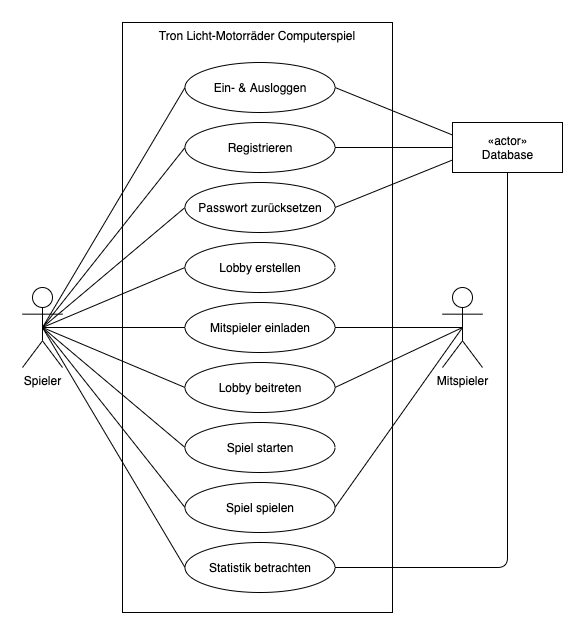
\includegraphics[scale=0.77]{figures/Use-case-modell.png}
            \caption{Anwendungsfalldiagramm - Tron Licht-Motorräder Computerspiel}
        \end{figure}

    \subsection{Hauptanwendungsfälle}
        Wir haben zwei Hauptanwendungsfälle identifiziert:
         \begin{itemize}
            \item Lobby erstellen
            \item Spiel spielen
        \end{itemize}
        Die Hauptanwendungsfälle werden in den nächsten zwei Abschnitten detailliert ausgeführt.

       \subsubsection{UC1: Lobby erstellen - \quotes{fully dressed}}
            \begin{tcolorbox}[enhanced, breakable, sharp corners, width=\dimexpr\textwidth-15mm\relax ,enlarge left by=10mm ,fontupper=\linespread{1.1}\selectfont, boxrule=1pt, title={UC1: Lobby erstellen}, colback=white, colframe=gray!22, coltitle=black]

                \textbf{Anwendungsfall:} Lobby erstellen \\
                \textbf{Ebene:} Anwenderziel \\
                \textbf{Primärakteur:} Spieler \\
                \textbf{Stakeholder und Interessen:}
                \begin{itemize}
                    \item \textit{Spieler}: Möchte mit anderen Spielern zusammen in einer Lobby beitreten oder seine eigene Lobby erstellen. Kann die Rolle des Lobby-Erstellers haben.
                    \item \textit{Mitspieler}: Möchten mit anderen Spielern zusammen in einer Lobby beitreten. Kann die Rolle des Lobby-Erstellers haben.
                    \item \textit{Lobby-Ersteller}:  Möchte das Spiel starten, wenn alle Spieler bereit sind.
                    \item \textit{System}: Möchte mehrere Spieler in einer Lobby haben, um ein Spiel starten zu können.
                \end{itemize}
                \textbf{Vorbedingungen:} Alle Spieler sind entweder mit einem persönlichen oder Gastkonto angemeldet.\\
                \textbf{Nachbedingungen:} Mehrere Spieler oder auch einzelne Spieler befinden sich in Lobbys. Das System ist in der Lage in den Lobbys mit mehreren Spielern ein Spielgang zu starten. \\
                \\  \textbf{Standardablauf:}
                \begin{enumerate}
                    \item Spieler/Mitspieler wechselt zur Lobbyansicht der Anwendung.
                    \item Spieler/Mitspieler wählt eine bestehende öffentliche Lobby aus.
                    \item Spieler/Mitspieler tritt diese Lobby bei.
                    \item Spieler und Mitspieler warten in Lobby auf weitere Mitspieler..
                    \item Spieler/Mitspieler klicken auf \quotes{Bereit}
                    \item Lobby-Ersteller startet das Spiel.
                    \item System überprüft ob alle Spieler in der Lobby bereit sind.
                \end{enumerate}
                \textit{Falls nicht alle Spieler bereit sind, muss der Lobby-Ersteller zu einem weiteren Zeitpunkt nochmals Schritt 6 ausführen. Erst wenn alle Spieler bereit sind, wird mit Schritt 8 fortgefahren.}
                \begin{enumerate}[resume]
                    \item System startet das Spiel.
                \end{enumerate}
                \textit{Es ist nun nicht mehr möglich - als Spieler oder Mitspieler - dieser Lobby beizutreten.} \\
                \textit{Spiel wird gespielt …, Ende des Spiels.}
                \begin{enumerate}[resume]
                    \item System öffnet Lobby wieder
                \end{enumerate}
                \textit{Spieler/Mitspieler können Lobby beitreten. Punkt 3 bis 9 wiederholen sich, bis Spieler sich entscheidet, das Spiel oder die Lobby zu verlassen.} \\
                \\ \textbf{Erweiterungen (oder alternative Abläufe):}
                \begin{itemize}
                    \item[2a.] Spieler können eigene Lobby erstellen:
                    \begin{enumerate}
                        \item Spieler klickt auf Lobby erstellen.
                        \item Spieler wählt ob die Lobby öffentlich zugänglich (public) ist oder nur für Freunde (private).
                        \item System erstellt eine Lobby.
                        \item System fügt den Spieler als Lobby-Ersteller der Lobby hinzu.
                    \end{enumerate}
                    \item[2b.] Spieler können privaten Lobbys von Freunden über einen Link beitreten:
                    \begin{enumerate}
                        \item Spieler öffnet Einladung.
                        \item Spieler öffnet den Link im Browser.
                        \item System fügt Spieler der Lobby des Freundes hinzu.
                    \end{enumerate}
                    \item[4a.] Spieler können Lobby verlassen:
                    \begin{enumerate}
                        \item Spieler/Mitspieler verlassen Lobby
                    \end{enumerate}
                    \item[4b.] Spieler/Mitspieler können weiter in der Lobby bleiben und weiterspielen:
                    \begin{enumerate}
                        \item Spieler/Mitspieler verlassen die Lobby nicht
                    \end{enumerate}
                \end{itemize}
                \textbf{Spezielle Anforderungen:}
                \begin{itemize}
                    \item Sobald ein Mitspieler der Lobby beigetreten ist, läuft ein Timer. Falls der Timer abgelaufen ist und der Mitspieler noch nicht bestätigt hat, wird dieser automatisch abgelehnt.
                    \item Maximale Spieleranzahl muss eingehalten werden. Es gibt eine obere Grenze von Mitspielern, die durch den Spieler definiert wird.
                    \item Internationalisierung der Sprache in den Textanzeigen.
                \end{itemize}

            \end{tcolorbox}

        \subsubsection{UC2: Spiel spielen - \quotes{fully dressed}}
            \begin{tcolorbox}[enhanced, breakable, sharp corners, width=\dimexpr\textwidth-15mm\relax ,enlarge left by=10mm ,fontupper=\linespread{1.1}\selectfont, boxrule=1pt, title={UC2: Spiel spielen}, colback=white, colframe=gray!22, coltitle=black]

                \textbf{Anwendungsfall:} Spiel spielen \\
                \textbf{Ebene:} Anwenderziel \\
                \textbf{Primärakteur:} Spieler \\
                \textbf{Stakeholder und Interessen:}
                \begin{itemize}
                    \item \textit{Spieler}: Möchte als letzter Spieler übrig bleiben
                    \item \textit{Mitspieler}: Möchte als letzter Spieler übrig bleiben.
                    \item \textit{Lobby-Ersteller}:  Möchte das Spiel starten, wenn alle Spieler bereit sind.
                    \item \textit{System}: Möchte alle Spieler - bereit zum spielen - in einer Lobby haben, um ein Spiel starten zu können.
                \end{itemize}
                \textbf{Vorbedingungen:} Mindestens 2 Spieler sind im Spiel.\\
                \textbf{Nachbedingungen:} Der letzte Spieler im Spiel wurde Sieger. Spiel wurde erfolgreich beendet. Lobby wird erneut angezeigt. \\
               \\  \textbf{Standardablauf:}
                \begin{enumerate}
                    \item System lädt Spiel.
                    \item System platziert Spieler/Mitspieler (Spielcharakter) in einem gewissen Abstand zum Spielfeldrand und zu den Mitspielern, jeweils in möglichst entgegengesetzter Richtung, auf dem Spielfeld.
                    \item System zeigt Countdown an. Nach Ablauf des Countdowns beginnt das Spiel.
                    \item System beginnt Startbewegung der Spieler mit konstanter Geschwindigkeit in Richtung Spielfeldmitte.
                \end{enumerate}
                \textit{Alle Spieler/Mitspieler auf dem Spielfeld behalten die konstante Geschwindigkeit bei bis zum Ausscheiden oder Ende des Spiels.}
                \begin{enumerate}[resume]
                    \item System erzeugt Hindernis vom Startpunkt des Spielers/Mitspielers bis zu dessen aktueller Position.
                    \item System übergibt Spieler/Mitspieler die Kontrolle des jeweiligen Spielcharakters.
                \end{enumerate}
                \textit{Schritt 4 - 6 folgen ohne Zeitverzögerung aufeinander.}
                \begin{enumerate}[resume]
                    \item Spieler/Mitspieler können, durch drücken einer Pfeiltaste, die Richtung um jeweils exakt 90\textdegree\ ändern.
                    \item Das durch den Spieler/Mitspieler erzeugte Hindernis, wächst mit der Bewegung und in der jeweiligen Bewegungsrichtung.
                \end{enumerate}
                \textit{Das vom Spieler/Mitspieler erzeugte Hindernis, bleibt auf dem Spielfeld bestehen bis zum Ausscheiden oder Sieg des Spielers/Mitspielers, in allen folgenden Schritten.}
                \begin{enumerate}[resume]
                    \item System koordiniert in kurzen Intervallen alle Bewegungen der Spieler/Mitspieler und überprüft deren Positionen und etwaige Kollisionen.
                \end{enumerate}
                \textit{System wiederholt Schritt 7 - 9 bis Kollision erkannt wird.}
                \begin{enumerate}[resume]
                    \item System entfernt Spieler/Mitspieler mit Kollision vom Spielfeld und zeigt eine entsprechende Meldung an.
                \end{enumerate}
                \textit{System wiederholt Schritt 7 - 10 bis ein einziger Spieler/Mitspieler auf dem Spielfeld übrig bleibt.}
                \begin{enumerate}[resume]
                    \item System zeigt bei letztem Spieler/Mitspieler eine Siegesmeldung an.
                    \item System beendet das Spiel.
                    \item System zeigt die Statistiken des Spiels bei allen Spielern/Mitspielern an.
                    \item System öffnet - nach Ablauf eines Timers  - erneut die Lobby.
                \end{enumerate}
                \textbf{Erweiterungen (oder alternative Abläufe):}
                \begin{itemize}
                    \item[?a.] blah
                        \begin{enumerate}
                            \item blah
                            \item blah
                            \item blah
                        \end{enumerate}
                \end{itemize}
                \textbf{Spezielle Anforderungen:}
                 \begin{itemize}
                    \item blah
                \end{itemize}

            \end{tcolorbox}

         \subsubsection{System-Sequenzdiagramm (SSD)}

    \section{Zusätzliche Anforderungen}

    \subsection{Funktionalität}

    \subsection{Benutzbarkeit}

    \subsection{Zuverlässigkeit}

    \subsection{Effizienz}

    \subsection{Änderbarkeit (Wartbarkeit)}

    \subsection{Internationalisierung}

    \subsection{Einschränkungen}

    \subsubsection{Designeinschränkungen}

    \subsubsection{Implementierungseinschränkungen}

    \subsubsection{Schnittstelleneinschränkungen}

    \section{Domänenmodell}

    \section{Softwarearchitektur}

    \section{Design-Artefakte}

    \section{Implementation}

    \section{Projektmanagement}


    % Appendix after this
     \newpage

    \section{Appendix}
    \textit{Hinweis: Glossar-Referenznummern sind Seitennummern}
    \printglossary

\end{document}

